% !TeX root = ./master.tex

\documentclass[12pt]{article}
\author{Gruppe 3}

\newcommand{\modulname}{Gas- \& Wasserstoffversorgung}
\newcommand{\semester}{WS 2021/2022}

%%%%%%%%%%%%%%%%%%%%%%%%%%%%%%%%%%%%%%%%%%%%%%%%%%%%%%%%%%%%
%
% Pakete
%
%%%%%%%%%%%%%%%%%%%%%%%%%%%%%%%%%%%%%%%%%%%%%%%%%%%%%%%%%%%%
\usepackage[ngerman]{babel} % Sprache deutsch
\usepackage{geometry} % Layout Geometrie
\usepackage[export]{adjustbox} % loads also graphicx
\usepackage[section]{placeins} % Floating
\usepackage{titleps} % Layout

% Notizen (zum Deaktivieren [disable])
\usepackage[textwidth=25mm,textsize=footnotesize]{todonotes}
\setlength\marginparwidth{1in}


% Schriftart
\usepackage{charter}

%%%%%%%%%%%%%%%%%%%%%%%%%%%%%%%%%%%%%%%%%%%%%%%%%%%%%%%%%%%%
%
% Style
%
%%%%%%%%%%%%%%%%%%%%%%%%%%%%%%%%%%%%%%%%%%%%%%%%%%%%%%%%%%%%
\newpagestyle{ruled}
{\sethead{\modulname}{- \thepage\space -}{Zusammenfassung}\headrule}
\pagestyle{ruled}

%%%%%%%%%%%%%%%%%%%%%%%%%%%%%%%%%%%%%%%%%%%%%%%%%%%%%%%%%%%%
%
% Befehle
%
%%%%%%%%%%%%%%%%%%%%%%%%%%%%%%%%%%%%%%%%%%%%%%%%%%%%%%%%%%%%
\newcommand{\vorlesung}[2]{
  \section{#1}
  {\small \textit{Vorlesung vom #2.}}\\[0.4cm]
}

\newcommand{\image}[2]{
  \begin{figure}[!htp]
    \centering
    \includegraphics[max height=19cm,max width=0.9\textwidth,keepaspectratio]{images/#1}
    \caption{#2}
    \label{image:#1}
  \end{figure}
  \FloatBarrier
} % Beispiel: \image{Funny.PNG}{Dies ist eine Beschreibung}

\begin{document}
  \begin{titlepage}
  \thispagestyle{empty}
  \newgeometry{right=0cm,left=0cm, top=0cm, bottom=0cm}
  
  \makebox[0pt][l]{
    \begin{picture}(50,50)
      % 100 vergrößern, damit logo hoch wandert 
      \put(543, -155){
        \hfill
        
\includegraphics[width=1.7cm]{./images/fh-logo-right.pdf} %fhac-right.pdf} %FHAC.jpg} 
      }
    \end{picture}
  }

  \begin{center}

    {\huge \textsc{\textbf{FH Aachen}}}\\[0.2cm]
    {\Large \textsc{University of Applied Sciences}}\\[0.2cm]
    
    {\Large \textsc{Fachbereich 10 - Energietechnik}}\\[0.5cm]
    {\Large \textsc{Energiewirtschaft \& Informatik (M. Sc.)}}\\
    {\Large \textsc{Energy Systems (M. Sc.)}}\\[2cm]

    {\Huge \textsc{\textbf{\modulname}}}\\[0.5cm]
    {\Large \textsc{Projektdokumentation - Gruppe 3}}\\[0.2cm]
    {\textsc{\semester}}\\
  \end{center}


  \vspace{1cm}

  \noindent\makebox[\textwidth][c]{
    \begin{minipage}{0.7\textwidth}
      \rule{\textwidth}{0.5pt}\\
      \begin{center}
        \LARGE \textbf{Modellierung und Analyse eines Energiesystemmodells  unter Berücksichtigung von CO2 Reduktionszielen}
      \end{center}
      \vspace*{.6cm}
      \rule{\textwidth}{0.5pt}\\
    \end{minipage}
  }


  \vspace{1.5cm}

  \begin{center}
    {\Large \textbf{Verfasser}}\\[0.5cm]
    {\Large Güllü Arslan}\\[0.2cm]
    {\Large Julien Tilly}\\[0.2cm]
    {\Large Melanie Ecker}\\[0.2cm]
    {\Large Paul Krüger}\\[0.2cm]
    {\Large Florian Steinberger}\\[0.2cm]
    {\Large Mehdi Abbadi}\\

    \vspace{2cm}

    Jülich, 07. Januar 2022
  \end{center}

 

  \end{titlepage}

  
  \tableofcontents % Inhaltsverzeichnis

  \newpage
  \listoffigures
  \listoftables
  
  \newpage
  \section{Einleitung}
\todo{Paul+Mel: Gewisse Wörter abkürzen? Abkürzungsverzeichnis}
\todo{Reduktionsfall, Reduktionsziel, Erneuerbare Energien, Photovoltaik, }
Weltweit haben in den letzten Jahrzehnten Naturkatastrophen aufgrund des menschenverursachten Klimawandels deutlich zugenommen. „Zwischen 2000 und 2009 waren es fünfmal so viele wie in den 70er Jahren“ \todo{ZITAT FLUTWELLE NRW 2021}
Eine statistische Auswertung hierzu ist in Abbildung \todo{Abbildung verlinken} zu sehen. Als Folgen des Klimawandels können Hitze- und Dürreperioden, Überschwemmungen, großflächige Waldbrände, schwerwiegende Stürme und häufige Extremwetterlagen beobachtet werden.
Damit das zusammenleben von Mensch und Planet Erde auch für die nächste Epoche gesichert ist, müssen neue Konzepte weg von fossilen Brennstoffen zu einer komplett auf erneuerbaren Energien konzipierten Energieversorgung entwickelt und in die Volkswirtschaften installiert
werden. Wichtig für die Konzeptfindung ist für die Entscheidungsträger dabei einen ganzheitlichen Überblick über die zu realisierenden Szenarien zu erhalten. Dies betrifft nicht nur die örtlichen Gegebenheiten für den Aufbau der Energiesysteme, sondern vor allem die entstehenden Kosten, die notwendige Logistik und notwendigen Ressourcen zur Installation und dem laufenden Betrieb der Anlagen. Im Lehrmodul Gas- und Wasserstoffversorgungsstrukturen wird als Projektarbeit eine solche Konzeptfindung für die zukünftige Energieversorgung der Bundesrepublik Deutschland einschließlich 100 \% CO2 Reduktion 2050 im Vergleich zu 1990 mit Simulationswerkzeugen Rechnerunterstützt mit Computer durchgeführt. Die nachfolgenden Seiten beschreiben die Ergebnisse der Simulationen und sollen allen Lesern einen schnellen Überblick über zukünftige Energieversorgungsszenarien plausibel darstellen. 

  \section{Modellbeschreibung}

Im praktischen Teil des Unterrichts im Fach Gas und Wasserstoffversorgungssysteme sollen zukünftige Energieverteilungsmodelle für Deutschland bei verschiedenen prozentualen CO2 Reduktionen im Vergleich zu 1990 mit damals emittierten 366 Mio. Tonnen simuliert werden. 

Basis der Simulationen stellt das vom Institut IEK3 des Forschungszentrums Jülichs bereitgestellten Framework „FINE“, welches die Programmiersprache Python implementiert und Energieszenarien mit Erzeugern, Verbrauchern und Speichern entwickeln und grafisch ausgeben kann.

Das verwendete Modell der Bundesrepublik wird dabei in acht Zonen als sogenannte Cluster von Null bis Sieben eingeteilt, welches in der Abbildung \ref{image:DEinCluster.png} zu sehen ist.
\todo{Cluster mit unterschiedlichen Nachfrage.. und Ausbaupotentialieln}

\image{DEinCluster.png}{Deutschland in 8 Cluster aufgeteilt}

FINE erzeugt nach Ablauf der Simulationen automatisch die Verteilung der Energiesysteme und Kopplung durch Pipelines und Stromtrassen inklusive einer visuellen Ausgabe der Ergebnisse.
Damit ein Vergleich der unterschiedlichen Teilnehmergruppen visualisiert und verglichen werden kann, benutzt jede Teilnehmergruppe in Ihrer Projektsimulation andere Energieversorgungs- und Verteilungskonzepte für Deutschland. Jedes Mitglied wird eine geforderte CO2 Reduktion zugewiesen, welche in den nachfolgenden Kapiteln von diesen präsentiert und erläutert werden.% In nachfolgender Tabelle XX sind die Reduktionen für die verschiedenen Simulationen zu sehen.


\begin{table}[]
    \begin{tabular}{|lcll|}
        \hline
        \multicolumn{4}{|c|}{Energiesystemdesign}                                              \\ \hline
        \multicolumn{1}{|l|}{Erneuerbare Energie Erzeugung} & \multicolumn{1}{l|}{Wind Onshore} & \multicolumn{1}{l|}{Wind Offshore} & Photovoltaik \\ \hline
        \multicolumn{1}{|l|}{Stromnetz AC}     & \multicolumn{3}{c|}{vorhanden}                \\ \hline
        \multicolumn{1}{|l|}{Stromnetz DC}     & \multicolumn{3}{c|}{vorhanden}                \\ \hline
        \multicolumn{1}{|l|}{H2 - Pipeline}    & \multicolumn{3}{c|}{vorhanden}                \\ \hline
        \multicolumn{1}{|l|}{Endenergiebedarf} & \multicolumn{3}{c|}{Strom und Wasserstoff H2} \\ \hline
    \end{tabular}
    \caption{Systemdesign}
    \label{tab:my-table}
\end{table}


Tabelle 2.2 zeigt das verwendete Konzept zur Simulationsausführung in FINE. Die
Bereitstellung aus erneuerbaren Energien stellen hierbei Windkraft in On- und Offshore
Konfiguration und Photovoltaik aus der direkten Sonnennutzung dar. Des weiteren existieren
Stromtrassen in Gleich- und Wechselstromkonfiguration und Pipelines zum Transport des
verwendeten Wasserstoffs zur Verfügung. Die Energieverbräuche der einzelnen Sektoren
werden in Form von Strom und direkter H2 Nutzung simuliert. Bestehende Wasserkraft,
Methan und Biogasanlagen werden in die Simulation mit einbezogen und der Einkauf von
zusätzlichen Ressourcen in Form Gasförmigen Stoffen angenommen. Weil in der Realität der
Ökonomische Gedanke stets eine Rolle spielt und keine Investitionen ohne die
wirtschaftlichen Parameter durchgeführt werden zeigt nachfolgende Tabelle XX die
verwendeten und kalkulierten Kosten zur Installation und Inbetriebnahme der
Energieressourcen in Deutschland. Das Framework „FINE“ bezieht diese Kenngrößen in die
Simulation mit ein und berechnet die Gesamten volkswirtschaftlichen Investitionskosten,
welche zukünftig zu treffen sind. 

%\image{tabelle_sonst.png}{Tabelle}

\begin{table}[h!]
    \centering
    \begin{tabular}{|ccl|}
    \hline
    \multicolumn{3}{|c|}{Parameter für die entstehenden Kosten der Simulation}                                          \\ \hline
    \multicolumn{1}{|c|}{\multirow{3}{*}{Wind Onshore}} & \multicolumn{1}{c|}{Investitionen} & 1,1 Mrd. € / GW Leistung \\ \cline{2-3} 
    \multicolumn{1}{|c|}{}                              & \multicolumn{1}{c|}{Operationen}   & 22 Mio. € / GW Leistung  \\ \cline{2-3} 
    \multicolumn{1}{|c|}{}                              & \multicolumn{1}{c|}{Lebenszyklus}  & 20 Jahre                 \\ \hline
    \multicolumn{1}{|c|}{\multirow{3}{*}{Wind Offshore}} & \multicolumn{1}{c|}{Investitionen} & 2,3 Mrd. € / GW Leistung \\ \cline{2-3} 
    \multicolumn{1}{|c|}{}                              & \multicolumn{1}{c|}{Operationen}   & 46 Mio. € / GW Leistung  \\ \cline{2-3} 
    \multicolumn{1}{|c|}{}                              & \multicolumn{1}{c|}{Lebenszyklus}  & 20 Jahre                 \\ \hline
    \multicolumn{1}{|c|}{\multirow{3}{*}{Photovoltaik}} & \multicolumn{1}{c|}{Investitionen} & 650 Mio. € / GW Leistung \\ \cline{2-3} 
    \multicolumn{1}{|c|}{}                              & \multicolumn{1}{c|}{Operationen}   & 13 Mio. € / GW Leistung  \\ \cline{2-3} 
    \multicolumn{1}{|c|}{}                              & \multicolumn{1}{c|}{Lebenszyklus}  & 25 Jahre                 \\ \hline
    \multicolumn{1}{|c|}{Gas / Methan}                  & \multicolumn{1}{c|}{Kaufpreis}     & 33.100 € pro GW Leistung \\ \hline
    \multicolumn{1}{|c|}{Biogas}                        & \multicolumn{1}{c|}{Kaufpreis}     & 54.090 € pro GW Leistung \\ \hline
    \end{tabular}
    \caption{entstehende Kosten}
    \label{tab:my-table}
    \end{table}
  \section{Durchführung der Rechenläufe}
Zur Modellierung des Energiesystemmodells wurde das Framework FINE von dem Forschungszentrum Jülich eingesetzt.
Dieses Framework ermöglicht die einfache Erstellung eines Energiemodells mit verschiedenen Regionen und Energiearten. Alle benötigten Komponenten, wie Energiequellen, Verbraucher, Speicher, Umwandler und Netze, können mit technischen und ökonomischen Merkmalen hinzugefügt werden. 

Das Framework FINE stellt das Jupyter Notebook ``Multi-regional\_Energy\_System\_Workflow.ipynb'' bereit, welches ein Energiesystem mit acht Regionen modelliert und optimiert. Das Notebook wurde entsprechend der Aufgabenstellung (siehe Kapitel TODO) angepasst.

Mithilfe des Gurobi Solvers wurde das Energiesystem hinsichtlich der Kosten unter Einhaltung der zuvor gesetzen Grenze für den CO2 Ausstoß optimiert. Das Ergebnis der Optimierung ist ein optimiertes Energiesystem, bei dem in jedem Zeitschritt die Nachfrage gedeckt und das CO2 Reduktionsziel eingehalten ist. Die Ausgabe von FINE ist vielseitig. Für jede Komponente und Region werden unter anderem die installierte Kapazität, der ``Fahrplan'' und die daraus resultierende Kosten ausgegeben.

Die Ausgabe der Optimierung wird in eine Excel-Datei exportiert, damit die Ergebnisse einfacherer analysiert und mit den Ergebnissen der anderen Reduktionsfällen verglichen werden können. 

Die Ausführung des Jupyter Notebooks für die sechs verschiedenen Reduktionsfälle wurde mithilfe eines Shell Scripts automatisiert. Das Script kopiert das Notebook, setzt das jährliche Limit für den CO2 Ausstoß entsprechend des Reduktionsfalles und führt das Notebook anschließend aus. Das Ergebnis ist eine Excel Datei je Reduktionsfall, welche anschließend zu einer übersichtlichen Excel zusammengefügt wird.
  \section{Analyse der Ergebnisse}
\label{sec:gesamtanalyse}

Im Folgenden erfolgt eine Gesamtbewertung für die einzelnen CO\textsubscript{2}-Restriktionen unter Berücksichtigung der jeweiligen Komponenten des Energiesystems. Im anschließenden Kapitel \ref{sec:reduktionsfaelle} wird dann noch mal die herausstechende Besonderheit je Reduktionsfall betrachtet. 

\subsection{Energiegewinnung}
Die unterschiedlichen Reduktionsziele stellen den Bedarf der Energieerzeugung aus erneuerbaren Energien dar. Insbesondere die Gewinnung aus Wind onshore, Wind offshore und Photovoltaik steigen signifikant, wobei der Anteil an Wind onshore kleiner ausfällt als die beiden anderen genannten. 

Betrachtet man die installierte Leistung für Wind onshore für den 75 \% Reduktionsfall liegt der Anteil bei 36 GW und reduziert sich bei 80 \% auf 23 GW. Ab einer CO\textsubscript{2}-Reduktion von 85 \% nimmt der Anteil wieder zu und steigt im 100 \% Szenario auf 44 GW. 
Dahingegen wird bei Wind offshore ein signifikant steigender Anteil ermittelt. Im 75 \% Reduktionsfall beträgt dieser 48 GW und steigt auf 81 GW bei einem Reduktionsfall von 90 \%. Dieser Wert ist scheinbar das Kapazitätsmaximum und bleibt daher bis zum 100 \% Szenario konstant.

Ein besonders hoher Anstieg ist bei der Energiegewinnung aus PV festzustellen. Beträgt dieser im Szenario 75 \% noch 30 GW, steigt er bei allen weiteren Reduktionsfällen ab 85 \% überproportional bis hin zu 188 GW installierter Leistung.

\smallimage{Erzeugung_EE.png}{Installierte Kapazität der EE je Reduktionsfall}

Die Erdgasverstromung aus GuD-Kraftwerken erhält in den ersten beiden Reduktionsfällen noch eine unverzichtbare Rolle mit einem Anteil von 56 \% im 75 \% Fall und mit 47 \% im 80 \% Fall. Bei den weiteren CO\textsubscript{2} Reduktionszielen verringert sich der Anteil kontinuierlich, bis dieser bei einem CO\textsubscript{2}-neutralen Energiesystem vollständig verschwindet. Dies ist damit zu begründen, dass bei der Verbrennung von insbesondere Erdgas viel CO\textsubscript{2} freigesetzt wird und sich somit negativ auf die CO\textsubscript{2}-Bilanz auswirkt. Anstelle des Erdgases wird deshalb in den Fällen mit höheren CO\textsubscript{2} Reduktionszielen auf Biogasanlagen gesetzt, da dabei kein CO\textsubscript{2} freigesetzt wird. 


\subsection{Energieumwandlung}
Bei der Energieumwandlung wird die Elektrolyse als wesentliche und unverzichtbare Größe dargestellt. Dabei ist die Elektrolyse so bedeutsam, weil sie die einzige Möglichkeit ist, um Strom in Gas umzuwandeln und so langfristig zu speichern.

Im betrachteten Energiesystem bleibt der Wert für den Einsatz der Elektrolyse für die ersten drei Reduktionsfälle gleich hoch. Ein Anstieg tritt ab dem 90 \% Fall ein und verdeutlicht die Notwendigkeit zum Ausbau der Elektrolyseleistung. Mit steigenden Reduktionsfällen wird mehr Leistung in der Elektrolyse benötigt, um die Erzeugungsspitzen aus erneuerbaren Energien zu berücksichtigen und den Bedarf der Wasserstoffherstellung zu decken. 

\smallimage{Elektrolyse.png}{Verlauf der Kapazität der Elektrolyse über die einzelnen Reduktionsfälle hinweg}

In allen Szenarien der CO\textsubscript{2}-Reduktion befindet sich die größte Kapazität der Elektrolyse in Region 6. Dies lässt sich vermutlich damit erklären, dass nur in Region 6 die Stromerzeugung durch Wind onshore stattfindet. Durch die Nähe von Erzeugern mit hohem Überschuss zu den Elektrolyseanlagen, kann der Strom direkt durch die Wasserstoffherstellung genutzt werden. In den Reduktionsfällen 75 \% und 80 \% ist Region 6 mit 11 GW die Einzige mit Elektrolyseanlagen.

In den Reduktionsfällen 85 \%, 90 \% und 95 \% gibt es zusätzlich eine Kapazität in Region 2. Die Investition in diese ist ähnlich zu erklären wie die Elektrolysenutzung in Region 6. Statt jedoch der Erzeugung aus Wind onshore, hat die Region 2 die größte Erzeugung aus Wind offshore.
Über die genannten Reduktionsfälle steigt dabei in beiden Regionen die Kapazität ähnlich stark an. 

In der 100 \%igen Reduktion von CO\textsubscript{2} sind für nahezu alle Regionen Elektrolyseanlagen vorgesehen. Lediglich Cluster 7 besitzt keine eigenen Anlagen und wird aus dem Pipelinenetz mit Wasserstoff versorgt. Die großen Kapazitäten liegen dabei weiterhin in Cluster 6 und 2.

\subsection{Energiespeicherung}
Die Energiespeicher erhalten bei steigenden Reduktionsfällen eine relevante Rolle. Der Bedarf resultiert aus dem notwendigen Ausbau der erneuerbaren Energien und der dazugehörigen Systemintegration. 
Dadurch können kurzfristige Übererzeugungen und Nachfrageschwankungen reguliert werden. 

In allen Szenarien ist ein Anstieg der Speichernutzung festzustellen, wie in Abbildung \ref{image:SpeicherDieSpeicher.png} zu sehen ist. H\textsubscript{2}-Salzkavernen und Biogas Salzkavernen erhalten neben Batteriespeichern und Pumpspeicherkraftwerken eine neue wichtige Rolle. Die Pumpspeicher werden in allen Reduktionsfällen bis zum Kapazitätsmaximum ausgelastet, erhalten jedoch mit steigender Reduktion eine deutlich höhere Nutzung. 
Aufgrund des Gasimports werden die Kavernen bei geringen Reduktionsfällen nicht berücksichtigt. Mit steigendem Reduktionsfall werden größere Speicher jedoch erforderlich.

\smallimage{SpeicherDieSpeicher.png}{Verlauf der Speichernutzung}

Ein Batteriespeicher speichert Strom kurzfristig und muss deshalb die Kapazität haben, um große Strommengen auf einmal zu speichern. Durch die beschränkte Größe sind Batteriespeicher in jeder Region möglich und auch immer im Einsatz.
Im Vergleich zu Batteriespeicher sind Pumpspeicherkraftwerke größer, da sie mithilfe von Wassermengen Strom mittelfristig speichern können. Pumpspeicher sind in allen Regionen bis auf Region 7 im Einsatz.
Die Speicher, die langfristig speichern, sind Kavernen. Diese benötigen jedoch einen unterirdischen Hohlraum, der als Speicher dienen kann. Die Gegebenheiten für einen solchen Speicher sind also nicht überall einfach zu finden. Kavernenspeicher für Biogas gibt es in Region 1, 2, 3 und 5, während Kavernenspeicher für H\textsubscript{2} in Region 1, 2, 3, 5 und 6 angesiedelt sind. In einigen dieser Regionen wird Strom aus Windenergie erzeugt, sodass der Überschuss in Gas umgewandelt und direkt eingespeichert werden kann.


\subsection{Energieübertragung}
Mit steigendem Reduktionsfall verhält sich die Wasserstoffnutzung eher konstant. Schon im 75 \% Reduktionsfall wird eine installierte Leistung mit 29 GW berücksichtigt. Um die erforderliche Menge und somit die Nachfrage bedienen zu können, ist der Ausbau des Pipelinenetzes erforderlich. Im 95 \% Reduktionsfall beträgt die Spitzenleistung 31 GW. Ein Rückgang der Leistung simuliert der 100 \% Fall mit einem Wert von 19 GW. In dem Zusammenhang spielt die Sektorkopplung eine große Rolle, wenn im Energiemodell die Emissionsreduzierung im Fokus steht. 

Der Strom wird in Form von Wechselstrom (AC) oder Gleichstrom (DC) über Leitungen transportiert. Die Kapazität von diesen bleibt über alle Reduktionsfälle hinweg gleich. Zwar ist nicht jede Region mit Leitungen für AC mit allen anderen Regionen direkt verbunden, aber es sind alle angeschlossen. Bei den Leitungen für DC haben nur die Regionen 0, 2, 4 diese.

\begin{figure}[!h]
    \begin{minipage}[b]{.4\linewidth} 
       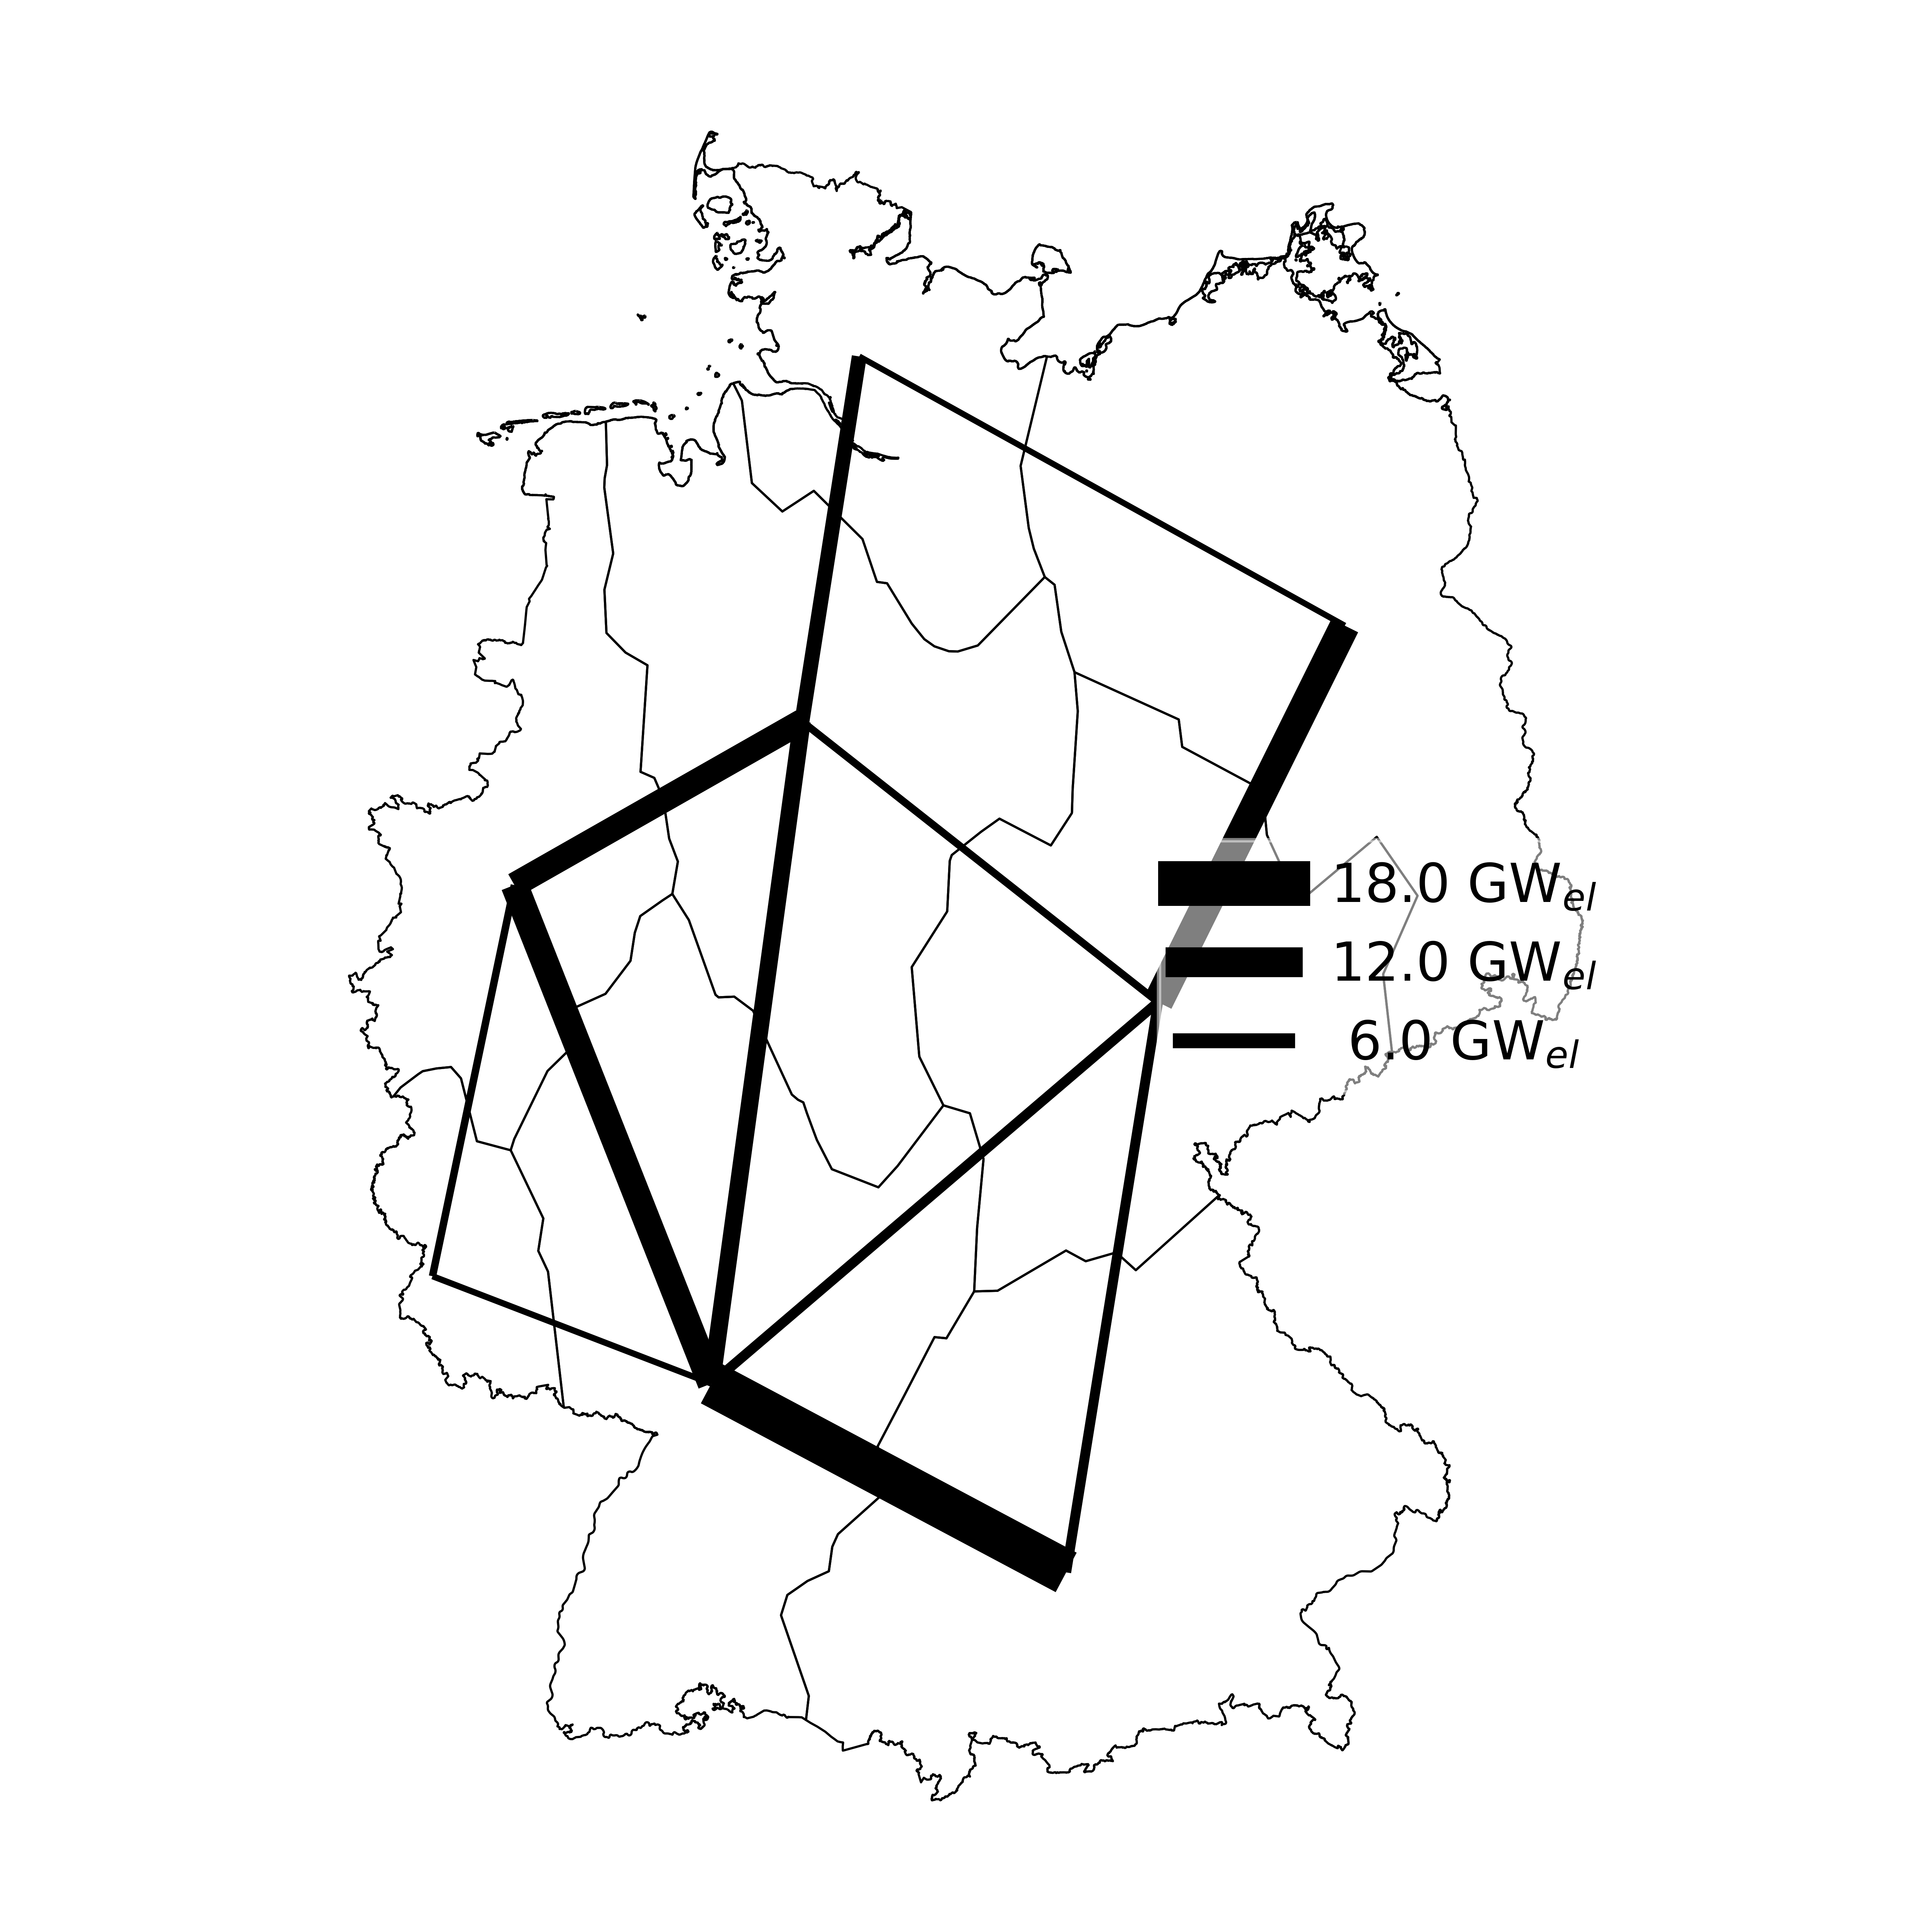
\includegraphics[width=\linewidth]{images/AC-insgesamt.png}
    \end{minipage}
    \hspace{.1\linewidth}
    \begin{minipage}[b]{.4\linewidth} 
       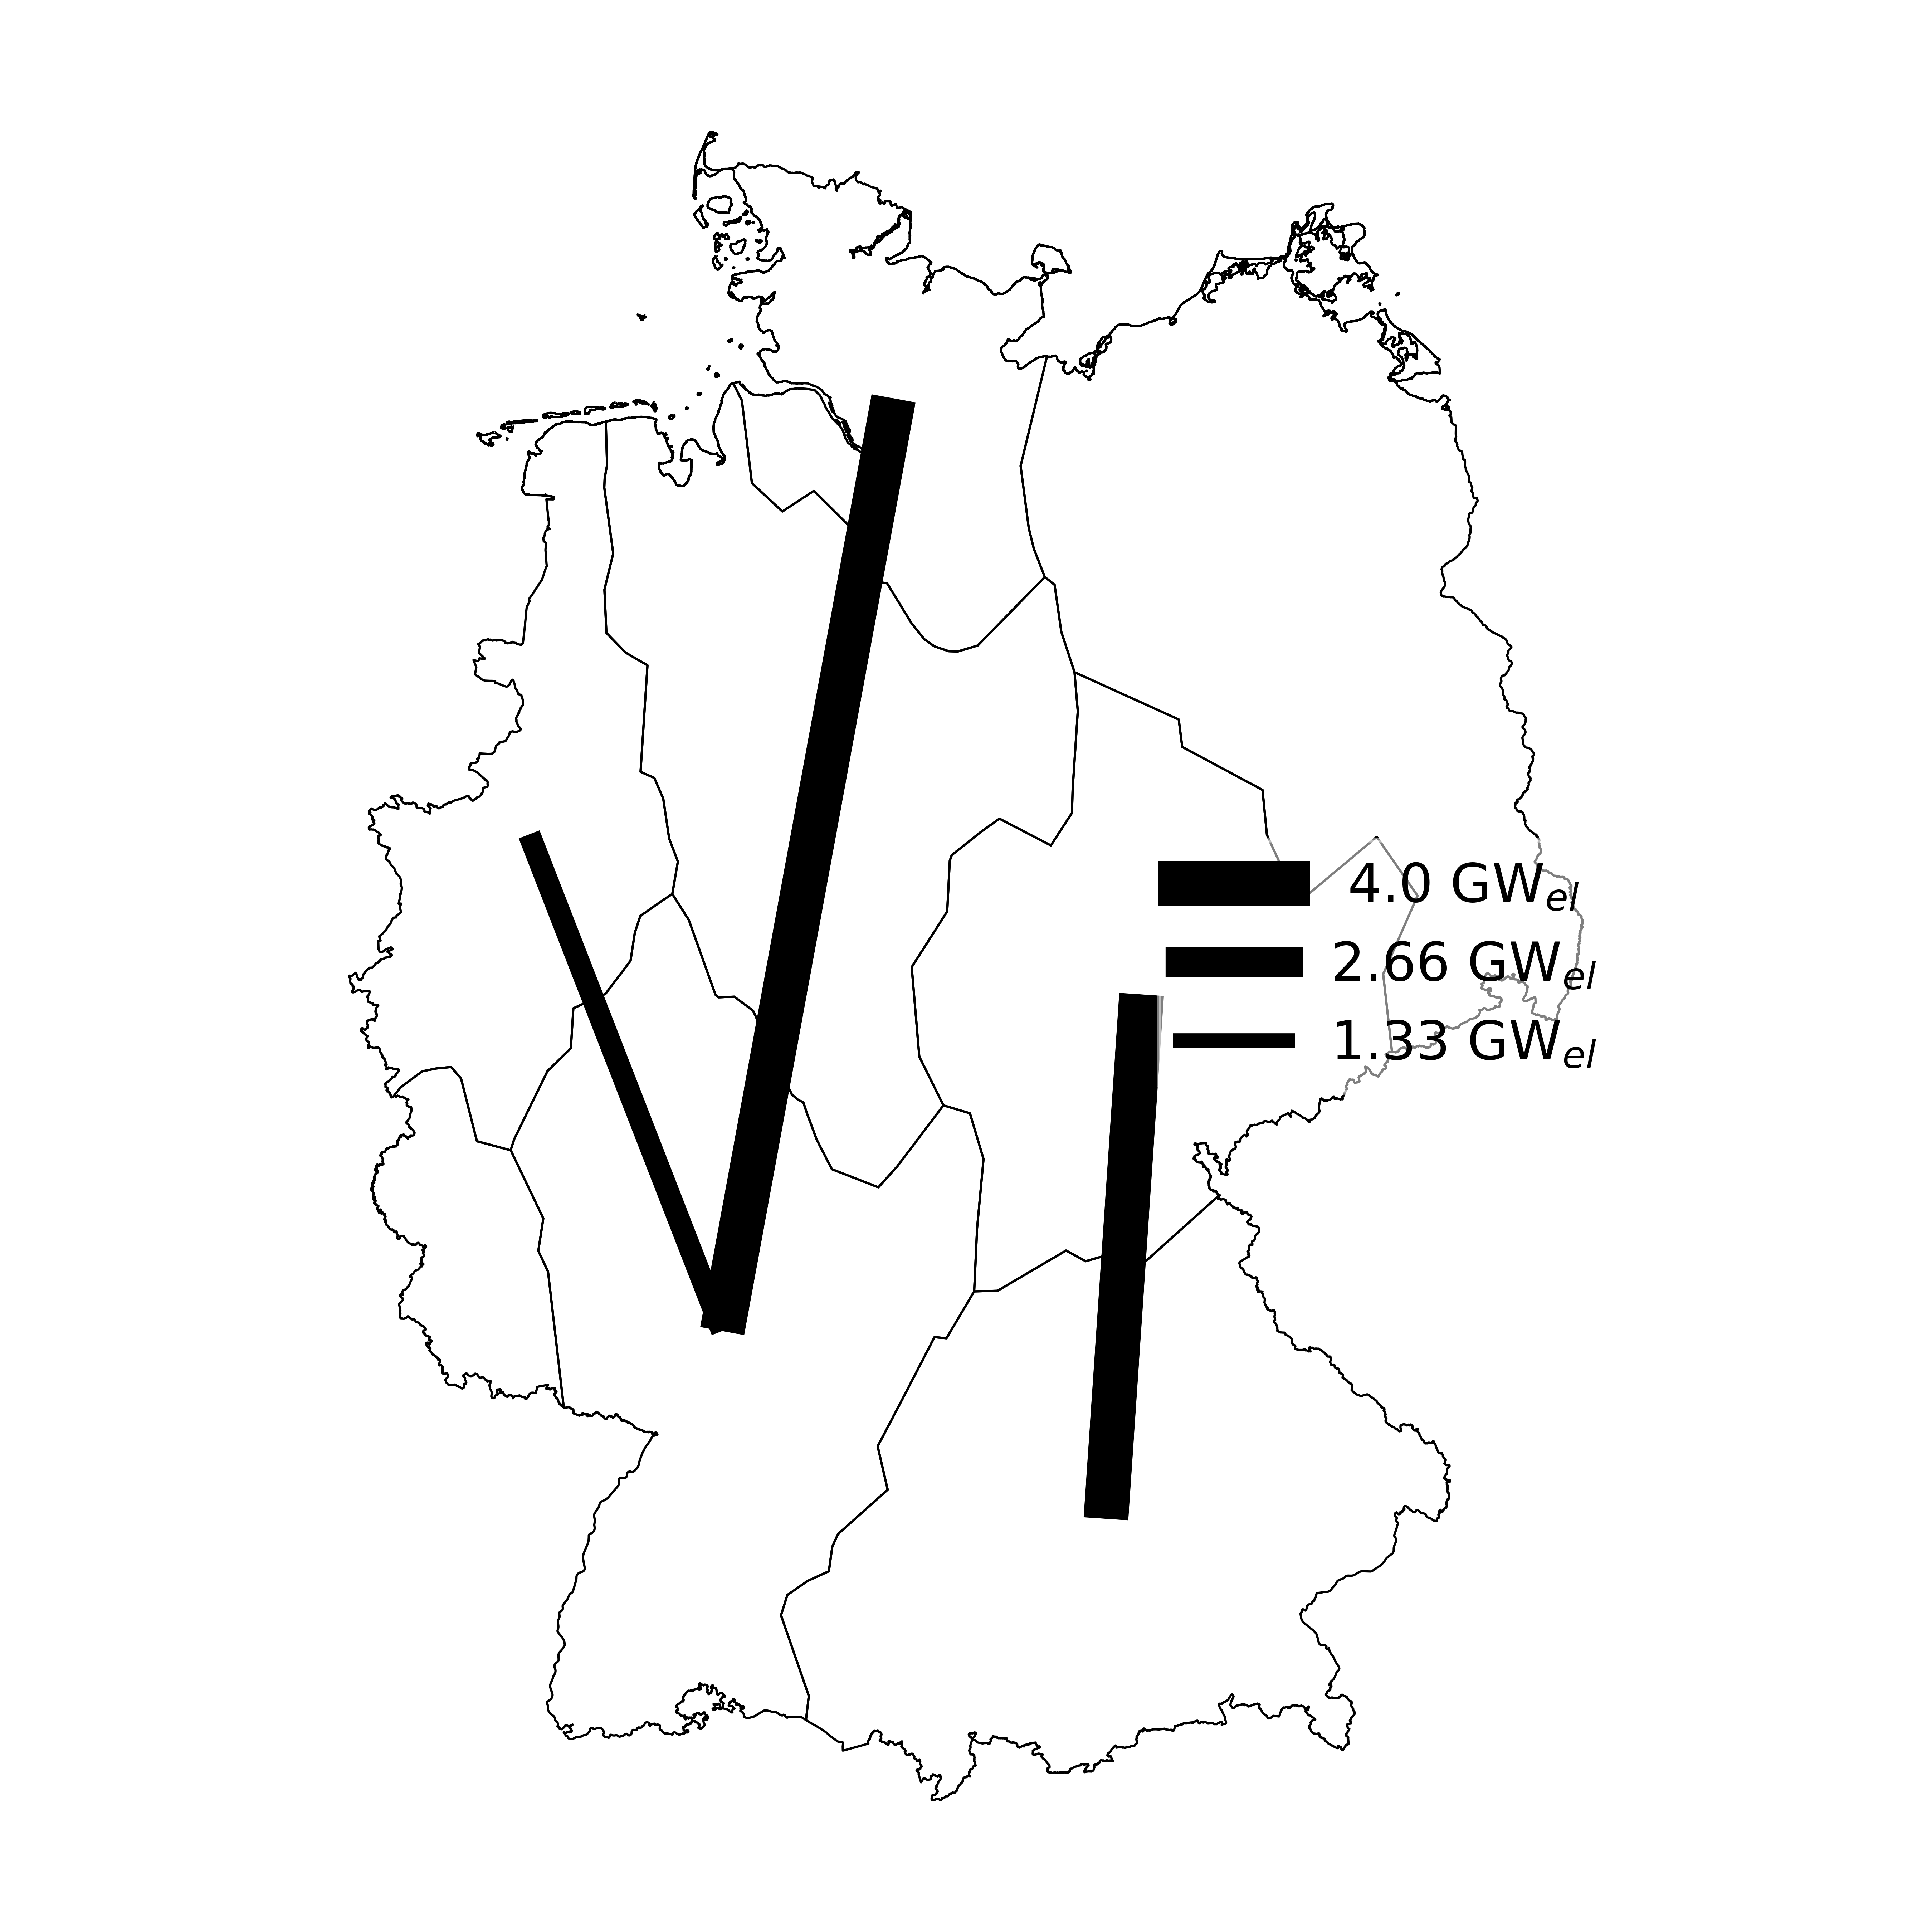
\includegraphics[width=\linewidth]{images/DC-insgesamt.png}
    \end{minipage}
    \caption{Lage der AC- und DC-Leitungen zwischen den acht Regionen}
    \label{image:Leitungen}
  \end{figure}


\subsection{Gesamtkosten (TAC)}
Für die Volkswirtschaft und die Zukunftsbetrachtung spielt die Kostenermittlung eine weitere Rolle. Als Kosten sind hier die Gesamtsystemkosten zu verstehen. Dabei handelt es sich im Wesentlichen um die fixen und variablen Betriebskosten, Investitionskosten und um die Importkosten. Im Rahmen der Projektarbeit und der zur Grunde liegenden Reduktionsfällen findet die Kostenoptimierung ebenfalls Berücksichtigung bei der Ausgestaltung des Energiemodells. Sollen Emissionswerte reduziert werden, impliziert dies die Einsparung fossiler Energieträger und führt somit zu einer Einsparung der Energiekosten. Berücksichtigt man alle für die Umsetzung erwähnten Komponenten für die unterschiedlichen Szenarien, belaufen sich die Gesamtkosten im 75 \% Fall auf ca. 41 Mrd. €/a und steigen im 100 \% Fall um 1,27 \% auf ca. 53 Mrd. €/a. Neben den Kosten für den Ausbau der Erzeugungsanlagen für erneuerbaren Energien, insbesondere Wind offshore und Photovoltaik, stellt der Wechsel von Erdgas Verstromung zu Biogas den großen Anteil dar. Der Anteil der Kosten zur Energieerzeugung beträgt bei ungefähr bei jedem Reduktionsfall 85 \% der Gesamtsystemkosten. Eine genaue Kostenaufteilung ist der Abbildung \ref{image:TAC.png} zu entnehmen. 

\smallimage{TAC.png}{Aufteilung der Gesamtkosten für das Energiesystem nach Reduktionsfall}

  \section{Analyse je Reduktionsfall}
\label{sec:reduktionsfaelle}
Nachdem im Kapitel \ref{sec:gesamtanalyse} die Komponentenbetrachtung im Fokus lag und grundlegende Aussagen getroffen wurden, wird nun der jeweilige CO2 Reduktionsfalls im Detail beschrieben und Besonderheiten hervorgehoben. Beginnend mit einer CO2 Reduktion von 75 \% folgen mit einer jeweiligen Änderung in fünfer Prozentpunkten die 80 bis 100 \% Fälle. In jeden Fall wird Bezug zu den ermittelten Werten genommen und eine Bewertung getroffen.

\todo{Alternativer Text, Paul}
Nachdem in Kapitel \ref{sec:gesamtanalyse} die Simulationen mit unterschiedlichen CO2 Reduktionszielen komponentenweise analysiert wurden, werden nachfolgend die verschiedenen Reduktionsfälle im Detail analysiert. In Tabelle \todo{ref} können die verschiedene Parameter der relevanten Kennzahlen für jeden Reduktionsfall übersichtlich dargestellt.


\todo{Prüfen, dass alle Zahlen mit Komma getrennt sind.}
\todo{Leerzeichen vor Prozent ja}
\todo{Einleitung schreiben}
\todo{Abbildung aller Reduktionsfälle + Bearbeiter}
\todo{CO2 mit tief gestellter 2 schreiben}

\subsection{75 \%}
Bei einem C02 Reduktionsziel von 75 \% belaufen sich die Gesamtkosten für das Energiemodell auf ca. 41 Mrd. €. Der Reduktionsfall zeichnet sich durch hohe Erdgasimporte aus. Aufgrund der geringeren CO2-Restriktion behält die Stromerzeugung von Erdgaskraftwerken noch eine signifikante Rolle. Die Zwischenspeicherung in Batteriespeichern ist in diesem Modell marginal. Der Rechenlauf berücksichtigt für das Energiemodell keine Kosten für den Einkauf von Biogas und somit entfällt auch der Bedarf an Biogasanlagen um innerhalb der Restriktion zu bleiben. 

Die Herstellung von Wasserstoff basiert auf Dampfreformierung und auf einheimische Wasserelektrolyse. In diesem Szenario wird der Bedarf an Wasserstoffspeicherung mittels Salzkavernen nicht in Anspruch genommen. UM die Treibhausreduktion um 75 \% zu schmälern, ist eine Langzeitspeicherung somit nicht erforderlich. Stattdessen ist festzustellen, dass zur Bedarfsdeckung von Wasserstoff der Ausbau der Pipeline zum Transport und Kurzspeicher vorhanden sein muss. 

Die installierte Leistung der Erzeugungsanlagen in dem Energiemodell beträgt 207 GW.  Der Anteil aus Windenenergieanlagen beträgt ca. 85 GW (Onshore 36 GW, Offshore 48 GW). Photovoltaikanlagen erzielen eine Leistung von knapp 30 GW. Die Differenz Leistung ist den anderen Erzeugungsanlagen im Modell zuzuordnen. 

Die Gesamtkosten teilen sich in 36,5 Mrd. € für Erzeugung, 4,7 Mrd. € für Umwandlung, 0,1 Mrd. € für Transport/ Übertragung auf. Da die Speicherung in diesem Reduktionsfall keine nennenswerte Rolle enthält, entstehen kaum Kosten. Aufgrund der vorausgesetzten Gegebenheiten sind die Kosten für die Erzeugung für das 75 \% Szenario im Verhältnis zu den anderen Szenarien am höchsten. 

Die Kosten für die Erzeugung fallen in dem 75 \% Szenario relativ hoch aus, was mit der Stromerzeugung aus Wind Offshore Anlagen zu begründen ist. Im Vergleich der Reduktionsfälle ist hier ein hoher Bedarf an Energiegewinnung aus Wind onshore Anlagen erforderlich, um die Nachfrage bedienen zu können. Den restlichen Bedarf wird mit der Stromgewinnung aus Photovoltaik, Gasanlagen und aus Laufwasserkraftwerken realisiert. Unter Optimierungsgesichtspunkten im Rechendurchlauf ist ein besonders hohes Augenmerk auf den erforderlichen Gasimport zu legen, welcher einen Anteil vom 56 \% an der Gesamtenergieerzeugung darstellt. Die genaue Aufteilung des Energiemixes kann der Abbildung \ref{image:Energiemix75.png} entnommen werden. Überschüsse sind in dem beispielhaften Energiesystem nicht berücksichtigt.
 

\smallimage{Energiemix75.png}{Reduktionsfall 75 \% - Mix Energiegewinnung}


\subsection{80 \%}
Die Gesamtsystemkosten betragen 42 Mrd. €. Sie steigen im Vergleich zum 75 \%-Reduktionsfall leicht an. Insbesondere die Kosten der Wind-Offshore-Anlagen (19 Mrd. €) steigerten sich um 6 Mrd. €. Diese Steigerung wird aber teilweise durch die sinkenden Erdgas-Importe ausglichen. Hierbei verringern sich die Kosten von 15 auf 12 Mrd. €. Dies lässt sich durch die Verringerung der CO2-Emissionen erklären. Die Kosten der restlichen Erzeugungsarten sinken um etwa 2 Mrd. €.

Werden die Gesamtsystemkosten nach Erzeugung, Umwandlung, Speicherung und Übertragung aufgeteilt, so liegt der Schwerpunkt bei der Erzeugung (37 Mrd. €). Die Umwandlung in den Elektrolyse-Anlagen ist mit 4,5 Mrd. € der zweitteuerste Kostenpunkt. Darauf folgt die Übertragung mit 123,7 Mio. Euro. Mit einem Anteil von 0,3 \% an den Gesamtkosten ist die Speicherung weit abgeschlagen.

Insgesamt beträgt die installierte Leistung der Erzeugungsanlagen 209 GW. Sie erfährt also eine Steigerung von 1,5 GW. Vermutlich lässt sich das auf die vermehrte Nutzung der Energiespeicher zurückführen. Die installierte Leistung Wind-Onshore geht auf 22,66 GW herunter. Die installierte Leistung Wind-Offshore nimmt stark zu. Ihr Wert beträgt 68,97 GW.  Weiter sinkt die installierte Leistung PV leicht auf 28,41 GW. Zudem bleibt die Elektrolyse-Leistung konstant auf 11,35 GW. 

Im gesamten Energiesystem werden 1.220.697,2 GWh/a erzeugt. Dabei überwiegen die erneuerbaren Energien mit einem Anteil von 53 \%. Erzeugung aus Erdgas ist im Vergleich zum 75 \%-Reduktionsfall um 10 \% zurückgegangen. Sie ist allerdings mit 47 \% noch im hohen Maße an der Energieproduktion beteiligt. Bei den regenerativen Energien stechen die Wind-Onshore Erzeugungsanlagen hervor. Diese haben zu 24,8 \% an der Gesamterzeugung und sind um 42,5 \% gegenüber dem 75 \%-Reduktionsfall angestiegen. 

Bei den Batteriespeichern gibt es eine Entwicklung. Ihre Speicherkapazität wächst auf 1,05 GWh an. Dies lässt sich vermutlich auf die geringere Nutzung der Gaskraftwerke zurückführen. Sie lassen sich nur noch vermindert für die kurzfristige Regelung im Netz einsetzten. Diese Aufgabe wird dann stärker von den Batteriespeichern übernommen. Ebenso finden die Pumpspeicherkraftwerke für die kurzen Lastspitzen Anwendung. Allerdings kann in den länger andauernden Dunkelflauten immer noch das importierte Erdgas eingesetzt werden. Dies führt dazu, dass weder H2- noch Biogas-Salzkarvenenspeicher eingesetzt. 

Die installierte H2-Pipelinekapazität steht unverändert bei 28,99 GW, da sich sowohl Kapazität der H2-Karvenenspeicher als auch die Elektrolyse-Leistung gleichgeblieben sind.

Sowohl bei den Kosten als auch bei der installierten Leistung hat die Offshore-Windkraft den größten Anteil. Hingegen gehen die Erzeugung aus Erdgas und die Importe des Erdgases zurück. Wobei 47 \% der erzeugten Energie weiter mit Erdgas produziert werden. Die restliche Erzeugung wird von erneuerbaren Energien gedeckt. Für kurzfristige Lastspitzen oder Engpässe werden vermehrt Batteriespeicher eingesetzt. Längerfristige Speicherung findet nicht statt, da keine Salzkarvenspeicher genutzt werden.


\subsection{85 \%}
Für den Reduktionsfall von CO2 um 85 \% würde das Gesamtsystem 43 Mrd. € kosten. Das System fokussiert sich dabei auf den Wechsel von Erdgas auf Biogas, von den Importen über die Gasanlagen bis hinzu den Speichern. Dabei werden erstmalig Biogasanlagen und die Speichermöglichkeit von Biogas in Salzkavernen genutzt.

Die Kosten des Gesamtsystems schlüsseln sich dabei auf in 38 Mrd. € für die Erzeugung, 4,3 Mrd. € für die Umwandlung, etwas weniger als 0,1 Mrd. € für die Speicherung und 0,1 Mrd. € für die Übertragung.

Im Vergleich zum Szenario mit 80 \% CO2 Reduktion haben sich die Kosten für die Erzeugung und Speicherung erhöht, während die Kosten der Umwandlung niedriger sind. Die Kosten für die Übertragung sind in etwa gleich geblieben. 
Insgesamt gibt es eine Erhöhung der Gesamtsystemkosten von ca. 1 Mrd. €. Dies kann u. a. durch die Reduktion der Gasanlagen mit Importen, Gasanlagen und Gasspeicher mit sinkenden Kosten und den erforderlichen Investitionen in Importe, Anlagen und Speicher für Biogas mit steigenden Kosten erklärt werden.

Das erstellte Energiesystem hat eine Gesamtkapazität von 200 GW Leistung durch Erzeugung und Umwandlung und eine Speicherkapazität von 510 GWh. Die Energie wird dabei zu 64 \% auf den erneuerbaren Energien und zu 36 \% aus Erdgas gewonnen. Mit 44 \% hat die Erzeugung durch Wind Offshore die größte Beteiligung am Energiemix, jedoch hat Natural Gas mit 37 \% auch noch einen großen Einfluss.

Es gibt einen steigenden Ausbau der Kapazität von Winderzeugung und PV-Erzeugung. Erstmalig wird in diesem Szenario Biogas importiert und Biogasanlagen genutzt. Weiterhin wird der Import und die Nutzung von Gasanlagen reduziert.

Genau wie beim Reduktionsfall von 80 \% ist die Kapazität für die Elektrolyse mit 11,35 GW gleichgeblieben.

Die Strommasse, die nicht verbraucht wird, kann kurzfristig in Batteriespeichern eingespeist werden. Diese wird in diesem Szenario auf 4,3 GWh ausgebaut und deren Kapazität hat sich vervierfacht.

Insgesamt ist die Speicherkapazität um 651 \% angestiegen. Die Speichernutzung für Pumpspeicher hat sich ungefähr um den Faktor 1,5 erhöht. Strom wird also öfter ein- und ausgespeichert, um dadurch die Extrema in der Lastkurve abzufangen. Zudem wird in diesem Energiesystem erstmalig Salzkavernen zur Speicherung von Biogas mit einer Speicherkapazität von 427,4 GWh verwendet.

Die installierte Kapazität der H2-Pipeline ist konstant geblieben, da die Leistung der Elektrolyse und der nicht vorhandenen Salzkavernen zur Speicherung von H2 nicht verändert wurde.

Beim Energiesystem im Reduktionsfall 85 \% ist Erdgas nicht mehr der größte Energieträger, stattdessen hat die Erzeugung durch Wind Offshore jetzt den größten Anteil.
Dadurch und durch den beginnenden Austausch von Natural Gas durch Biogas, sowie der Speicherung von Biogas in Kavernen und der generellen höheren Speichernutzung werden die CO2-Emissionen um 85 \% reduziert.

\subsection{90 \%}
Der Reduktionsfall 90 \% zeichnet sich dadurch aus, dass dieser als einziger untersuchter Reduktionsfall ohne Batteriespeicher zur Bereitstellung kurzfristig verfüg\-barer Flexibilität auskommt. Dies ist durch einen Salzkarvernenspeicher für Wasserstoff möglich, der in diesem Reduktionsfall erstmalig verwendet wird. Durch den Speicher kann die Herstellung von Wasserstoff durch Elektrolyse von der Wasserstoffnachfrage entkoppelt werden. Die Elektrolyse kann dadurch die erforderliche Flexibilität in dem Stromnetz bereitstellen.

Zur Erreichung der CO2 Reduzierung um 90 \% im Vergleich zu dem Jahr 1990 muss die Verbrennung von Methan in GuD-Kraftwerken weiter reduziert werden. Denn dies ist in dem Energiesystem der einzige Anlagentyp, bei dem CO2 freigesetzt wird. Im Vergleich zu dem Reduktionsfall 85 \% wird der Methan Import um 33 \% auf 182.090 GWh LHV gesenkt. Die maximale Leistung der GuD-Kraftwerke zur Umwandlung von Methan zu Strom sinkt um 19 \% auf 81,8 GW. Die unterschiedlichen prozentualen Rückgänge zwischen Methan Import und GuD-Kraftwerken lässt darauf schließen, dass der Stellenwert von GuD-Kraftwerken als flexible Energiegewinnungsanlage zur Sicherung von Versorgungsengpässen in diesem Szenario weiterhin hoch ist.

Der Anteil von Methan Importen als Quelle zur Energiegewinnung sinkt in diesem Energiesystem auf 25 \%. Die entstehende Lücke wird durch den weiteren Zubau von erneuerbaren Erzeugungsanlagen kompensiert. Der Ausbau von Offshore Windenergie steigt auf 81 GW und könnte damit unter Berücksichtigung der vorherrschenden Winde maximal 352.067 GWh Strom in dem simulierten Jahr erzeugen. Tatsächlich werden 346.158 GWh erzeugt. Dies bedeutet, dass die installierte Leistung zu 98,3 \% genutzt wird.
Photovoltaikanlagen werden in nahezu allen Clustern zugebaut, um die wegfallenden GuD-Kraftwerke zur Verbrennung von Methan zu ersetzen. Die installierte Leistung beläuft sich auf 60,2 GW (Zuwachs von 30 \% gegenüber dem vorherigen Reduktionsfall) und die Anlagen werden unter Berücksichtigung der maximalen Sonneneinstrahlung zu 99,5 \% ausgenutzt.
Die Wind Onshore Anlagen werden in diesem Reduktionsfall ausschließlich in Cluster Sechs mit einer Leistung von 29,8 GW installiert und erzeugen 76.283 GWh Strom (Ausnutzung der Anlage von 94,3 \%). Auch bei den GuD-Kraftwerken zur Biogas Verbrennung steigt der Anteil zum Ausgleich der fehlenden Energiegewinnung aus Methan an. \todo{Mehr Biogas. Aufgrund des Rückbaus steigende Relevanz für Versorgungssicherheit}
Die genaue Aufteilung der Energiequellen für das Energiesystem kann der Abbildung \ref{image:Energiemix90.png} entnommen werden.
Die Kosten für die Energiegewinnung belaufen sich auf 39,6 Mrd. €.

\smallimage{Energiemix90.png}{Reduktionsfall 90 \% - Mix Energiegewinnung}

In diesem Szenario wird Wasserstoff ausschließlich durch die Elektrolyse gewonnen, da Brennstoffzellen zu teuer wären.
Die Gesamtkosten zur Energieumwandlung betragen 4,4 Mrd. € und schließen die Kosten für die GuD-Kraftwerke für Methan und Biogas mit ein.
Der Ausbau von Onshore Windenergie nur in Cluster Sechs ist mit der Elektrolyse und dem damit verbundenen Strombedarf zu begründen. 
Elektrolyseure wird ausschließlich in den Clustern Zwei und Sechs mit einer Leistung von 18 GW betrieben. Die dafür erforderliche Energie stammt nahezu ausschließlich von Onshore und Offshore Windparks in den jeweiligen Clustern. Dies erfordert Flexibilität im Energiesystem, denn das Angebot an Strom aus Windenergie entspricht nicht der Nachfragekurve für Wasserstoff. 

Der erstmals installierte Salzkarvernen für Wasserstoff können die Energie zwischen Angebot und Nachfrage zwischenspeichern. Die Elektrolyseure können dadurch ausschließlich die überschüssige Windenergie zur Umwandlung nutzen und stellen dadurch die im Stromnetz benötigte Flexibilität bereit. Ein Batteriespeicher wird dadurch in diesem Energiesystem nicht benötigt.
Der Salzkarvernenspeicher kann maximal 2.241 GWh LHV Wasserstoff speichern und wird im simulierten Jahr zur Speicherung von 19.725 GWh LVH eingesetzt. Dies bedeutet, dass die Wasserstoffnachfrage zu 23 \% aus dem Speicher bedient wird. Der Salzkarvernenspeicher sind in sind aufgrund der räumlichen Nähe zur Wasserstofferzeugung in den Clustern Eins, Zwei und Sechs installiert.
Aufgrund der Importbegrenzungen von Biogas ist auch ein Salzkarvenenspeicher zur Zwischenspeicherung zwischen Import und Verbrennung im GuD-Kraftwerk erforderlich. Aus diesem Speicher werden die saisonalen Schwankungen in Strom-Erzeugung und Nachfrage gedeckt.
Wie auch bei den anderen Reduktionsfällen wird der Pumpspeicher zum Ausgleich der täglichen Schwankungen in der Stromnachfrage genutzt. 
Die Gesamtkosten für Energiespeicherung belaufen sich auf 1,3 Mrd. €.

\smallimage{Installed_hydro_pipelines_0.9.png}{Reduktionsfall 90 \% - Übertragungsnetz für  Wasserstoff}

Übertragungsnetze ermöglichen die räumliche Trennung zwischen Energieerzeugung und Energienachfrage. 
Aus ökonomischer Sicht ist es sinnvoll, dass Energiespeicher und Energieerzeugung in räumlicher Nähe zueinander gebaut werden. Denn dadurch können die gleichen Übertragungsnetze für den Transport zu den Nachfragern genutzt werden, unabhängig davon ob die Nachfrage durch die Erzeugungsanlagen oder aus dem Speicher bedient wird. 
Die installierten Pipelinekapazitäten zwischen allen Regionen sind in Summe 30,9 GW. Die Verbindung zwischen Cluster Eins und Sechs ist aufgrund der notwendigen Speicherbefüllung mit 7,7 GW am Größten.
Das erstellte Pipelinenetz für die Verteilung von Wasserstoff kann der Abbildung \ref{image:Installed_hydro_pipelines_0.9.png} entnommen werden. Das gesamte Übertragungsnetz kostet 129 Mio. €.

Auch wenn die Verbrennung von Methan eine vergleichsweise günstige und flexible Energiegewinnung ermöglicht, muss dieser Anteil zur Erreichung des Reduktionsziels deutlich gesenkt werden. Die fehlende Erzeugung wird durch die erneuerbaren Energien aufgefangen, die die hohe Flexibilität nicht mehr gewährleisten können. Zur Aufrechterhaltung der Versorgungssicherheit sind deshalb andere Erzeuger oder flexible Verbraucher erforderlich. In diesem Reduktionsfall wird neben den Pumpspeichern vermehrt auf Biogas GuD-Kraftwerke gesetzt und erstmals durch einen Energiespeicher die Elektrolyseure als flexible Verbraucher in dem Stromnetz eingebunden.
Zur Erreichung des Reduktionsziels von 90 \% wurde ein Energiesystem mit Gesamtkosten von 45 Mrd. € durch das Framework FINE erzeugt.

\subsection{95 \%}

\smallimage{Energiemix95.png}{Reduktionsfall 95 \% - Gesamtenergieverteilung bei 95 \% Reduktion im Jahr 2050}

In oben zu sehender Abbildung \ref{image:Energiemix95.png} ist die grafische Auswertung der CO2 Reduktion bei 95 \% in den jeweiligen Anteilen an der Gesamtenergieverteilung zu sehen. Im Vergleich zum vorherigen Unterkapitel von 90 \% wird die Erhöhung der CO2 Reduktion nun durch gesteigerte Anteile an Offshore Windkraft und Photovoltaik erreicht. Die Anteile an Solarzellen werden dabei von 9 \% auf 19 \% um weitere 10 \% erhöht, während die Anteile der Offshore Windkraft lediglich um weitere 2 \% von 48 \% auf 50 \% gesteigert werden. Die jeweiligen Anteile an importiertem Biogas, der Laufwasserkraftwerke, der Onshore Windkraft und den importierten Natural Gasen bleiben im Vergleich zu 90 \% unverändert. 
Die Nachfolgende Abbildung \ref{image:KapazitätWind-95.png} veranschaulicht die grafische Verteilung der Offshore Windkraft an elektrisch installierter Leistung in GW. Der größte Anteil wir dabei mit etwa 50 GW an der Nordseeküste von Niedersachsen von Fine installiert, währenddessen sich um Schleswig-Holstein Nord- und Ostseeküsten in etwa der mittlere Anteil von etwa 20 GW befindet. Die niedrigen Anteile an Offshore Windkraft stellen hierbei die Ostseeküste um Brandenburg und ein großer Anteil der verbliebenen Küstengebiete von Schleswig-Holstein und Niedersachsen mit etwa bis zu 5 GW installierter elektrischer Leistung zur Verfügung. Insgesamt ermittelte Fine die Anteile von 50 \% Offshore Windkraft mit einer elektrischen installierten Leistung von etwa 81 GW. Die Kosten der Installation werden mit 22,7 Milliarden € kalkuliert. Bezogen auf Gesamtinstallationskosten von 47,96 Milliarden € entspricht dies einen Kostenanteil von 47,33  \%. Der Leistungsbeiwert bzw. Wirkungsgrad von Windkraftanlagen kann dabei über 50 \% erreichen. \todo{Fußzeile - Quelle:Energiezukunft.EU. (15. 05 2021). Von https://www.energiezukunft.eu/erneuerbare-energien/biomasse/wirkungsgrade-flaechenverbrauch-und-emissionen/ abgerufen} 

\smallimage{KapazitätWind-95.png}{Reduktionsfall 95 \%}

Der zweite große Anteil der Photovoltaik an der erneuerbaren Energieversorgung wird mit einer gesamt installierten Leistung von 120 GW von FINE kalkuliert. Monokristalline Solarzellen erreichen heute einen Wirkungsgrad von etwa 22 \% \todo{Fußzeile - Quelle:Energiezukunft.EU. (15. 05 2021). Von https://www.energiezukunft.eu/erneuerbare-energien/biomasse/wirkungsgrade-flaechenverbrauch-und-emissionen/ abgerufen}  und können flächendeckend auf allen Hausdächern, Bushaltestellen, Fabriken und neuen Versuchen mit solar betriebenen Geh- und Fahrradwegen installiert werden. Aktuell sind in Deutschland etwa 53,58 GW elektrische Leistung installiert \todo{Fußzeile - Quelle:Energiezukunft.EU. (15. 05 2021). Von https://www.energiezukunft.eu/erneuerbare-energien/biomasse/wirkungsgrade-flaechenverbrauch-und-emissionen/ abgerufen} . Das erneuerbare Energien Gesetz sieht allein bis 2030 eine Steigerung auf bis zu 100 GW vor.\todo{Fußzeile - Quelle:Energiezukunft.EU. (15. 05 2021). Von https://www.energiezukunft.eu/erneuerbare-energien/biomasse/wirkungsgrade-flaechenverbrauch-und-emissionen/ abgerufen}  Die in unserer Fine Simulation ermittelte Photovoltaik Leistung von ungefähr 121 GW bis zum Jahr 2050 kann dabei durchaus als realistisch betrachtet werden. Nachfolgende Abbildung \ref{image:KapazitätPV-95.png} zeigt die Verteilung der zukünftigen Solaranlagen in Deutschland. Den niedrigsten Solaren Anteil platziert FINE nun in den Süd Westlichen Regionen um Baden-Württemberg, dem Saarland und Teilen von Hessens mit etwa insgesamt 5 GW installierter Leistung. Die Weitaus größten Teile werden von der Simulation im Bereich von Mitteldeutschland um Nordrhein-Westfalen, Niedersachsen, Hessen, Thüringen und den Teilen der Bundesländer um Sachsens mit Gebieten um die 20 GW im Osten bis zur maximal 35 GW im Westen implementiert. Bayern im Süden und Schleswig-Holstein im Norden erhalten in etwa jeweils 10 GW bis 15 GW an solaren Anteilen. Bezogen auf den wesentlich geringeren Wirkungsgrad der Solarzellen im Vergleich zu Windkrafträdern lassen sich somit auch die deutlich höheren installierten Leistungen von 121 GW PV zu den 81 GW Offshore Windkraft erklären. Die Kosten der PV Installation belaufen sich dabei auf ca. 8,9 Milliarden €, welche einem prozentualen Anteil von ca. 18,5  \% an den Gesamtkosten entsprechen.

\smallimage{KapazitätPV-95.png}{Reduktionsfall 95 \%}

\smallimage{Speicher-95.png}{Reduktionsfall 95 \% - Energiespeicherkapazitäten der Simulation bei 90 \% und 95 \% CO2 Reduktion}

Abbildung \ref{image:Speicher-95.png} veranschaulicht nun die Simulierten Energiespeicher bei 90 \% und 95 \% CO2 Reduktionen. Waren bei 90 \% noch keine Batteriespeicher vorgesehen ermittelt Fine nun bei 95 \% bereits notwendige Batteriespeicher mit einem Speichervolumen von 4,42 GWh. Die Wasserstoff Salzkavernen verdoppeln sich nahezu in ihren Speichervermögen von 1664,55 GWh auf 3735,46 GWh, währenddessen der Anteil an Kavernen mit Biogas nahezu unverändert bleibt und nur einen minimalen Zuwachs erfahren. Der Anteil an Pumpspeichern ist zur vorherigen Simulation unverändert geblieben. 

\subsection{100 \%}
%\renewcommand{\reduktion}{100}
%\newpage
\section{CO\textsubscript{2} Reduktionsfall \reduktion\space\%}

\begin{tabularx}{0.5\textwidth} { 
  | >{\raggedright\arraybackslash}X 
  | >{\centering\arraybackslash}X | }
 \hline
 TAC [1e9 Euro/a] (Gesamtsystemkosten) & 42  \\
 \hline
 Installierte Leistung Wind-Onshore/ Wind-Offshore/ PV in den Regionen (je nach Gruppenvorgabe) [GW] & 42  \\
 \hline
 Installierte Leistung Elektrolyse [GW] & 42  \\
 \hline
 Speicherkapazität Batteriespeicher [GWh] & 42  \\
 \hline
 H2 Salzkavernen Speicherkapazität [GWh] & 42  \\
 \hline
 Installierte H2 Pipelinekapazität gesamt [GW] & 42  \\
 \hline
\end{tabularx}

Die Gesamtsystemkosten betragen 52 Mrd. €. Sie steigen im Vergleich zum alle Reduktionsfälle an. Insbesondere die Kosten der Wind-Offshore-Anlagen (22 Mrd. €) steigerten sich um 6 Mrd. €. Diese Steigerung wird aber teilweise durch die sinkenden Erdgas-Importe ausglichen. Hierbei verringern sich die Kosten von 15 auf 12 Mrd. €. Dies lässt sich durch die Verringerung der CO2-Emissionen erklären. Die Kosten der restlichen Erzeugungsarten sinken um etwa 2 Mrd. €.

Die Kosten der Wind-Offshore Anlagen sind massiv gestiegen im Vergleich zur Anfang Szenario (22 Mrd. €), somit steigen die Gesamtsystemkosten in höchst Szenario , betragen 52 Mrd. Dies ist ersichtlich da , die Kosten für den Gas-Import sinken . Diese Steigerung  ist auch wegen von verschiedene Speicherkapazitäten wobei die H2 Salzkavernen zum Einsatz ab dem 85 \% Fall zur Speicherung von Wasserstoff.

Die Kostenaufteilung im 100 \% Fall, nach Erzeugung, Umwandlung, Speicherung und Übertragung. Der Größte Anteil der Gesamtkosten besteht in der Erzeugung von ca. 86 \% (45 Mrd. €) als Schwerpunkt, der zweite Anteil ist durch die Speicherung zu sehen mit ca. 9 \% der Gesamten kosten (4,5 Mrd. €), danach kommen die Elektrolyse-anlagen mit ca. 2,93 Mrd. €. Die Umwandlungskosten liegen bei ca. 5,6 \% des TAC. Die restlichen 0,2 \% sind für die Übertragung geeignet.

Die gesamte installierte Leistung beträgt in allen Erzeugungsanlagen 370GW., mit einer Steigerung von ca. 50 GW zu den vorherigen Reduktionsfall. Dies kann aufgrund der massive Produktion aus der Erneuerbare Energie passieren. Da der Anteil an PV riesig angestiegen von 121 GW auf 188,2 .Die installierte Leistung an Wind-Offshore steigt  auf 81 GW als Spitzenwert, was macht lohnend bei Überschüsse, Elektrolyseanlagen nah zu den Clustern mit mehr Energie auszubauen.  Die installierte Leistung Wind-Onshore beträgt ca 44,2GW. Die Elektrolyse-Leistung steigt somit . auf den Wert maximal  23,3GW.

Bei den Batteriespeichern gibt es eine massive Steigerung. Die Speicherkapazität nimmt stark zu auf  129,46 GWh an. Dies lässt sich auf die Speicherbedarf , da die EE speisen viele Energie im Netz ein. Die Speicherung  wird dann stärker von den Batteriespeichern und von Gas Salzkavernen übernommen. Die Pumpspeicherkraftwerke haben eine deutliche geringere  Anwendung, unterscheidet sich aber nach Reduktionsfall. Dies führt dazu, dass der Einsatz von  H2- und Biogas-Salzkarvenenspeicher wichtig ist. Da deren Speicherkapazität enorme Beträge haben.

  \section{Fazit}
Anhand des Modells konnte dargestellt werden, dass die unterschiedlichen Szenarien zum Teil und insbesondere in Abhängigkeit der Treibhausreduzierungsziele, stark voneinander abweichen. Der Anwender kann sich mit Hilfe dieses Programms ein Bild über die erforderlichen Maßnahmen bis zur 100 %igen CO2-Neutralität machen. 
Festzuhalten ist der überproportionale Bedarf an Energie, der die Grundlage für das zu entwickelnde Energiesystem darstellt. Daneben stellen die PtX-Anlagen ein weite-res wichtiges Element zur Sektorenkopplung dar, um den Wasserstoffbedarf neben Importen selber zu decken. 
Die ambitionierten CO2 Ziele der Bundesregierung lassen aus heutiger Sicht eine nicht Erreichung mutmaßen. Umso wichtiger erscheinen die daraus gewonnenen Erkenntnisse, um den Wert annähernd zu erreichen. Der Stromerzeugungsmix wird als zwingende Voraussetzung ermittelt, so dass der Ausbau der erneuerbaren Ener-gien einen sehr hohen Stellenwert hat. Somit wird die Zubaurate an EE in den Folge-jahren signifikant steigen müssen. 
Neben der Erzeugung kann der Speicherung von H2 und Energie eine tragende Rolle zugesprochen werden. Die Erschließung der Speicher an das Energiesystem in Deutschland ermöglichen eine Langzeitspeicherung und unterstützen die Treibhausreduktionsziele. 

\end{document}